%%%%               %%%%
%%%% PLANIFICACIÓN %%%%
%%%%              %%%%

\chapter{Planificación}
\label{chap:planificación}

\lettrine{E}{n} este capítulo se aborda la planificación del proyecto.

\section{Recursos necesarios}

Para acometer el proyecto son necesarios varios tipos de recursos:

\begin{itemize}
    \item Recursos humanos
        \begin{itemize}
            \item Director del proyecto para los roles de Product Owner.
            \item Analista para las fases de análisis del proyecto.
            \item Diseñador para las fases de diseño del proyecto.
            \item Equipo de desarrollo formado por el alumno. Para la parte de integración se colaboró con otro alumno del Laboratorio de Telemática, pero no intervino en ningún momento en la creación de esta parte del proyecto.
        \end{itemize}
    \item Recursos software: todos los recursos software utilizados son aplicaciones sin coste monetario. Muchas son, además software libre.
    \item Recursos hardware: el portátil, pantalla y otros accesorios utilizados.
\end{itemize}

\subsection{Planificación económica}

De los recursos utilizados para el proyecto se deducen directamente los costes económicos incurridos. El cálculo de los costes salariales está extraído del \emph{Convenio colectivo del sector de empresas de ingeniería y oficinas de estudios técnicos} en su página del BOE \footnote{\url{https://www.boe.es/diario_boe/txt.php?id=BOE-A-2019-14977}}.

\begin{table}[ht]
    \centering
    \begin{tabular}{l l l l}
        Recurso & Coste (€/h) & Tiempo (h) & Coste total (€) \\
        \hline
        \hline
        Jefe de proyecto & 42 & x & x \\
        Analista & 35 & x & x \\
        Diseñador & 35 & x & x \\
        Programador & 30 & x & x \\
        Equipamiento informático & -- & x & 900 \\
        Software & -- & - & 0 \\        
        \hline
        \hline
        TOTAL & & - & x \\        
    \end{tabular}
    \label{Tab:costes-proyecto}
    \caption{Costes del proyecto}
\end{table}

\section{Planificación temporal inicial}

En la imagen \ref{fig:gantt-inicial} se presenta el diagrama de Gantt inicial de la planificación con el desglose de tareas. Una de las dificultades para la planificación consistió en no saber en qué momento del proyecto sería necesario abordar la integración con la interfaz web. En este plan inicial se contemplaban 524 horas de trabajo.

\begin{figure}[hp!]
    \centering
    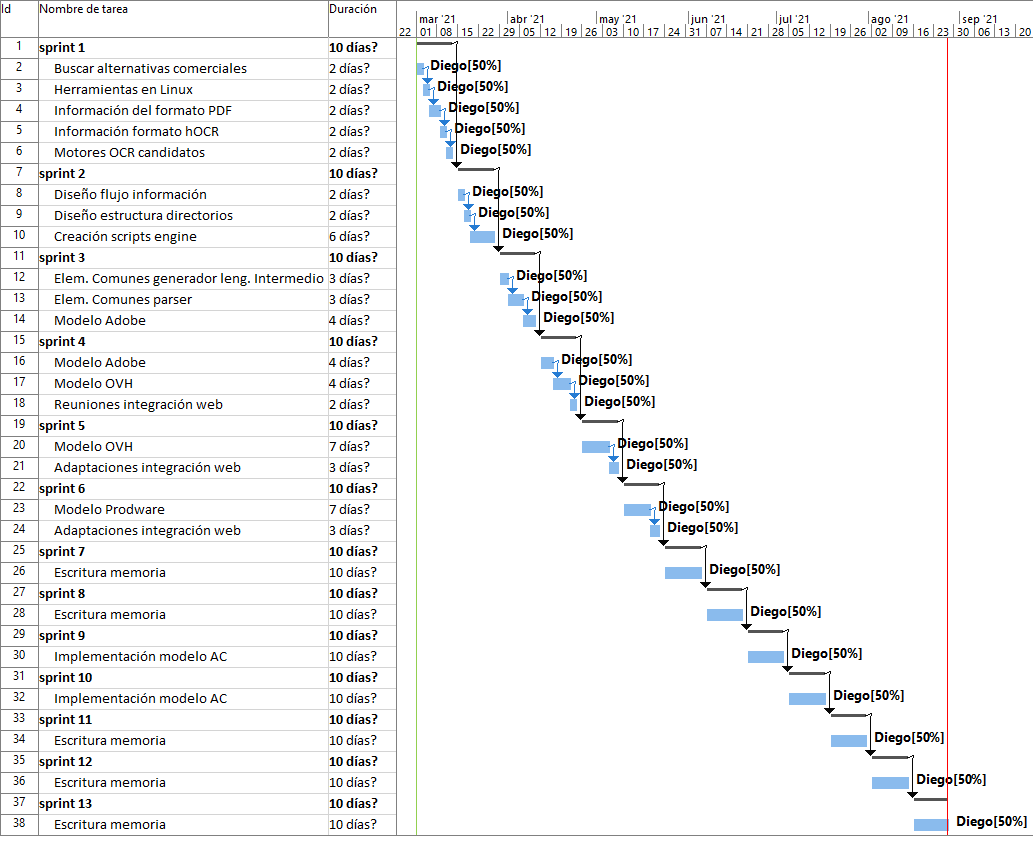
\includegraphics[angle=90,width=1.0\textwidth]{imaxes/f-planificacion/gantt-inicial.png}
    \caption{Diagrama de Gantt y tareas iniciales del proyecto}
    \label{fig:gantt-inicial}
\end{figure}

\section{Sprints}

Se expone acontinuación la distribución del trabajo a lo largo de los sprints. Por motivos de compatibilidad con el trabajo y responsabilidades personales, se escogió una fórmula de 20 horas de trabajo semanal y una duración de cada sprint de 2 semanas.

\subsection{Sprint 1}

Este primer sprint se dedicó completamente a la búsqueda de información, análisis del problema y diseño de alto nivel de la solución. Este periodo se utilizó para conocer las herramientas para tratar PDF disponibles en Linux, entender mejor el formato PDF, encontrar la existencia de los formatos de información de los procesos de OCR, hOCR; y búsque

Este primer sprint consistió por completo en un spike con el objetivo de recabar toda la información necesaria para plantear el proyecto a nivel técnico. Principalmente se buscó información de

\begin{itemize}
    \item Información de alternativas comerciales en la misma temática
    \item Herramientas disponibles en Linux para tratar PDF.
    \item Información del formato PDF.
    \item Información sobre hOCR
    \item Motores de OCR candidatos para el proyecto
\end{itemize}

\subsection{Sprint 2}

Con el conocimiento de reunido se procedió a la construcción inicial del sistema para el procesamiento por lotes de los trabajos. Además de diseñar la estructura de directorios utilizada por el proyecto, se crearon el Makefile, utilizado para las compilaciones y los scripts para implementar el motor.

\subsection{Sprint 3}

El sprint 3 se creó el generador de lenguaje intermedio y el primer parser para el modelo de documento de Adobe.

\subsection{Sprint 4}

En este sprint se añadió soporte para generación de código intermedio y parsing del modelo de OVH. También tuvieron lugar las primeras reuniones de trabajo para explicar el proyecto y decidir las adaptaciones necesarias de cara al prototipo.

\subsection{Sprint 5}

Se completó el modelo de documento del proveedor Prodware. Además se abordaron de forma paralela las tareas relacionadas con el prototipo web. Hubo varias reuniones para facilitar la implemtación de aspectos que no habían sido considerados, como  la necesidad de generar imágenes de las páginas individuales de cada documento, cambio del formato de la marca de tiempo y dockerización de la aplicación.

\subsection{Sprints 6, 7 y 8}

En estas tres semanas se abordó la escritura de la memoria, con el plan de dejar tiempo al final del proyecto para poner el punto y final.

\subsection{Sprint 9}

Implementación de los modelos basados en imagen.

\subsection{Sprint 10}

Implementación de los modelos basados en imagen.

\subsection{Sprint 11}

El sprint 11 se utilizó para construir el prototipo del editor de coordenadas.

\subsection{Sprint 12 y 13}

Los últimos dos sprints se dedicaron a finalizar la escritura de la memoria.


\section{Planificación temporal final}

% TODO explicar que las reuniones se adelantaron a las fechas previstas
